\documentclass[dvips,11pt,a4paper]{article}

\usepackage[danish]{babel}
\usepackage[utf8]{inputenc}
\usepackage{amsmath}
\usepackage{amssymb}
\usepackage{graphicx}
\usepackage{subcaption}

%%
%% Set non-standard dimensions for the page layout
%%
\setlength{\hoffset}{0pt}
\setlength{\voffset}{0pt}
\setlength{\oddsidemargin}{0pt}
\setlength{\evensidemargin}{0pt}
\setlength{\textwidth}{16cm}
\setlength{\topmargin}{-37pt}
\setlength{\textheight}{670pt}
\setlength{\footskip}{60pt}


\title{Generering af PAM-signaler i MATLAB}
\author{Lars Staalhagen (larst@fotonik.dtu.dk)}
\date{\today}

\begin{document}

\maketitle

\noindent{}Dette dokument beskriver, hvordan MATLAB's indbyggede foldningsfunktion, \texttt{conv()}, på en nem måde kan benyttes til at generere et tidsdiskret (dvs. samplet) PAM\footnote{PAM =  Puls Amplitude Modulation.}-signal; populært også kaldet et ''pulstog''. 

\section{Kontinuerte PAM-signaler}
Et (tids-)kontinuert PAM-signal kan helt generelt defineres som i formel~(\ref{eq:pamanalog}), hvor det er forudsat, at første informationssymbol, $a_0$, genereres til $t=0$, og dermed at der ikke ønskes sendt information før $t=0$.
\begin{equation}
v(t)=\sum_{k=0}^{\infty} a_{k} \cdot g(t-k \cdot T)
\label{eq:pamanalog}
\end{equation}

\noindent{}I formel~(\ref{eq:pamanalog}) indgår følgende:
\begin{itemize}
\item $a_k$ er informationssymbolerne ($k=0,1,2,\ldots$)
\item $g(t)$ er en funktion, der beskriver pulsen som funktion af tiden, $t$.
\item $T$ er symbolperioden, dvs. tidsintervallet mellem to $a_k$-symboler skal sendes.
\end{itemize}

\noindent{}Et eksempel på en simpel pulsform er en \emph{firkantformet} puls, $g(t)$ af varighed $T$, illustreret i figur~\ref{fig:pam003}, som kan defineres ligning~(\ref{eq:squarepulse}).
\begin{equation}
g(t) = \left\{
	\begin{array}{ll}
	1 & \mathrm{for}\quad{}0 \le t < T \\
	 & \\
	0 & \mathrm{ellers}\\
	\end{array}
	\right.
\label{eq:squarepulse}
\end{equation}

\begin{figure}[htbp]
\centering
\scalebox{0.7}{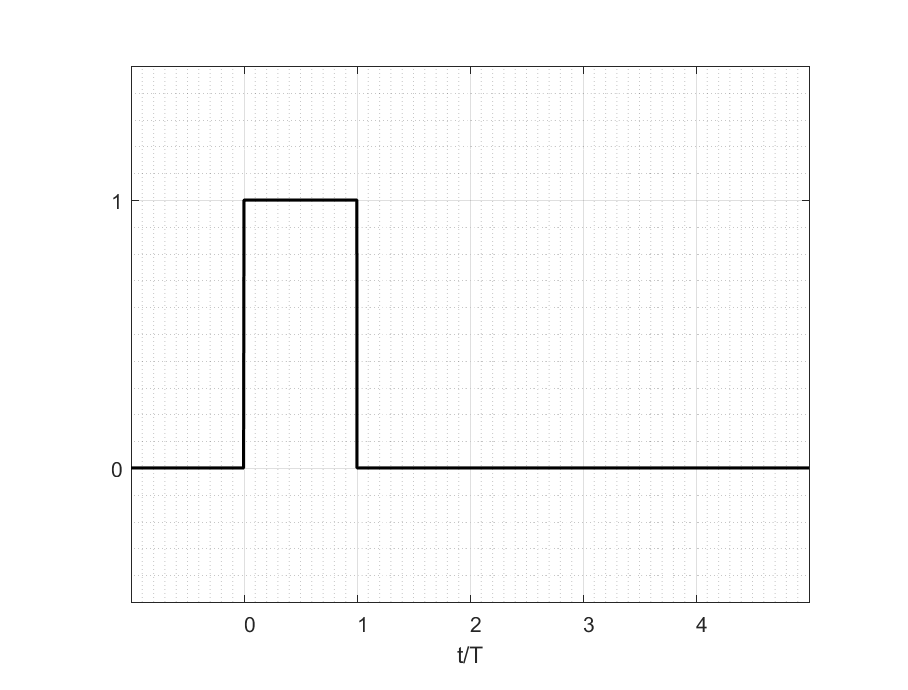
\includegraphics{pam003}}
\caption{\label{fig:pam003}Firkantpuls.}
\end{figure}

\noindent{}Grunden til, at funktionen for pulsformen i formel~(\ref{eq:pamanalog}) har argumentet $t-k\cdot{}T$ er, at det ''forskyder'' pulsen, afhængig af nummeret (indeks) på informationssymbolet, $k$.  Figur~\ref{fig:pam002} illustrerer udtrykket $g(t-k\cdot{}T)$ for $k=0,1,2,3$, for pulsen i ligning~(\ref{eq:squarepulse}) og det kan ses, at grundpulsen ''forskydes'' $k\cdot{}T$ til højre -- jo større $k$-værdi, jo mere er pulsen ''forskudt''.
\begin{figure}[htbp]
\centering
\scalebox{0.7}{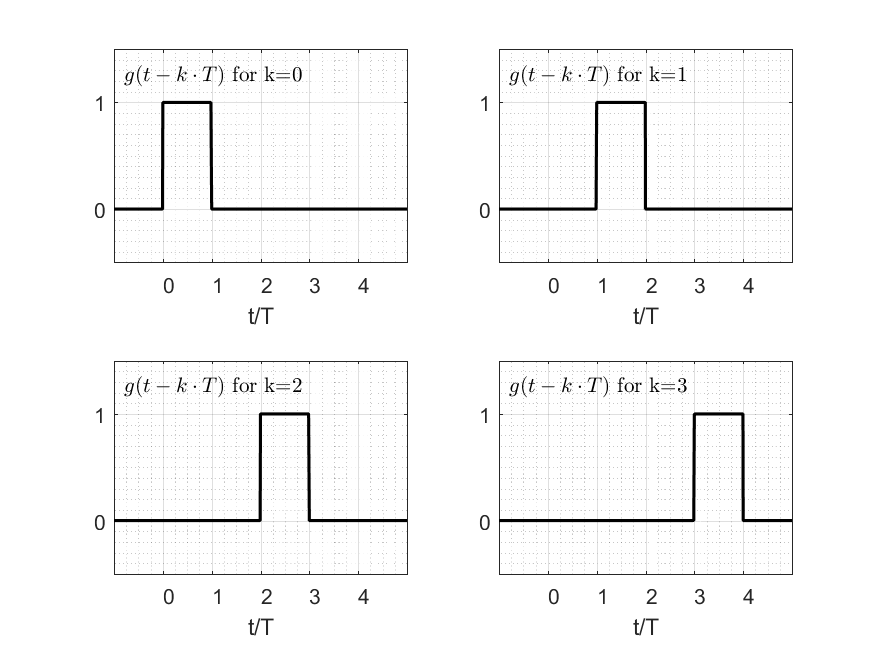
\includegraphics{pam002}}
\caption{\label{fig:pam002}Udtrykket $g(t-k\cdot{}T)$ for $k = 0,1,2$ og $3$.}
\end{figure}

Figur~\ref{fig:pam001a} illustrerer et simpelt PAM-signal, hvor der skal transmitteres informationssekvensen $a_{k} = +1,+3,-1,+1,-3,+1$, ved at benytte den firkantformede puls fra ligning~(\ref{eq:squarepulse}).
\begin{figure}[htbp]
\centering
\scalebox{0.7}{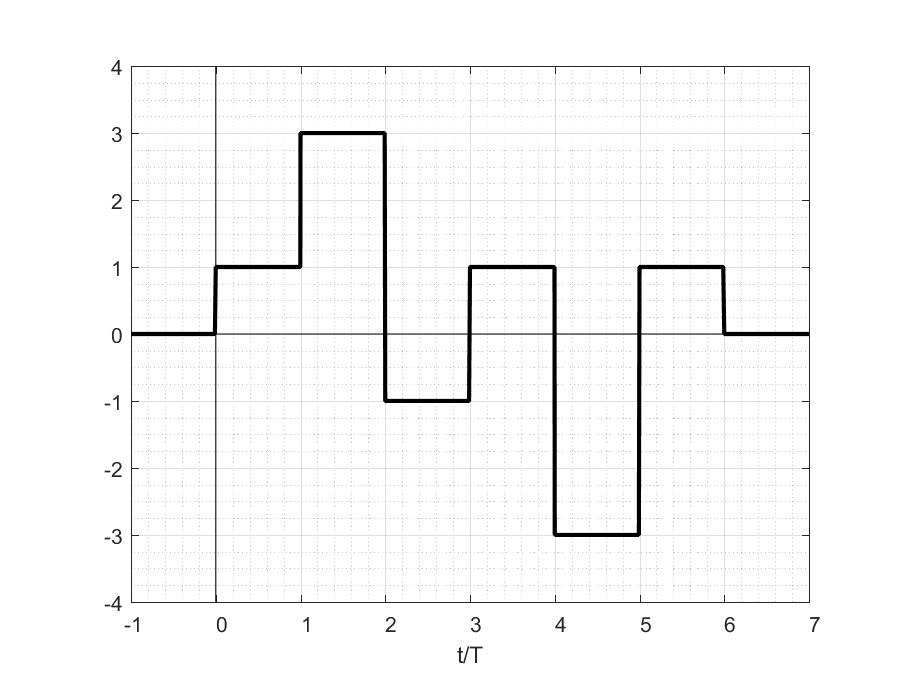
\includegraphics{pam001a}}
\caption{\label{fig:pam001a}Kontinuert PAM-signal med firkantformet puls.}
\end{figure}

Et PAM-signal kan dog også dannes ud fra andre pulsformer end firkantformede. Et eksempel er en ''savtak''-formet puls, der kan defineres som i ligning~(\ref{eq:sawtoothpulse}), og figur~\ref{fig:pam001c} viser et PAM-signal med samme informationssekvens som ovenfor, men nu med den savtakformede puls i ligning~(\ref{eq:sawtoothpulse}).
\begin{equation}
g(t) = \left\{
\begin{array}{ll}
t/T & \mathrm{for}\quad{}0 \le t < T \\
& \\
0 & \mathrm{ellers}\\
\end{array}
\right.
\label{eq:sawtoothpulse}
\end{equation}
\begin{figure}[htbp]
\centering
\scalebox{0.7}{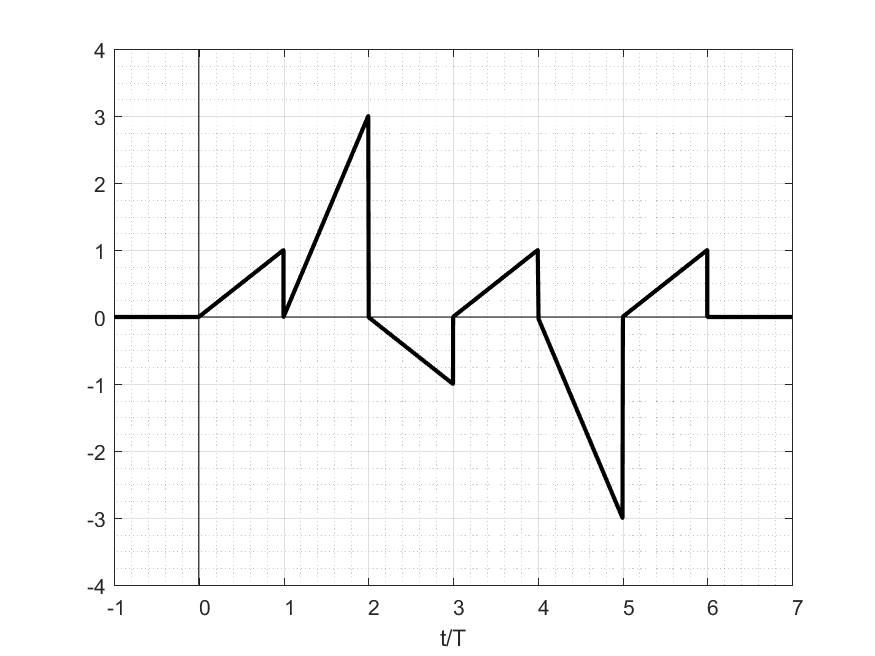
\includegraphics{pam001c}}
\caption{\label{fig:pam001c}Kontinuert PAM-signal med savtakformet puls.}
\end{figure}

\section{Tidsdiskrete PAM-signaler}
I digitale kommunikationssystemer er man imidlertid kun interesseret i signalerne til diskrete tidspunkter, dvs. de analoge signaler er blevet digitaliseret (dvs. samplet og kvantiseret) og vi er derfor kun interesseret i værdierne til tidspunkterne $t = n \cdot T_{s}$, hvor $T_s$ er samplingsintervallet og $n = 0,1,2,\ldots$. 

En tidsdiskret udgave af ligning~(\ref{eq:pamanalog}) fås derfor ved at erstatte $t$ med $n \cdot T_s$ i ligning~(\ref{eq:pamanalog}):
\begin{equation}
v(n \cdot T_{s})=\sum_{k=0}^{\infty} a_{k} \cdot g(n \cdot T_{s}-k \cdot T)
\label{eq:pamdiskret2}
\end{equation}

\noindent{}Figur~\ref{fig:pam001bd} viser de tidsdiskrete udgave af PAM-signalerne i hhv. figur~\ref{fig:pam001a} og figur~\ref{fig:pam001c}, hvor der i begge tilfælde er samplet 4 gange inden for hver symbolperiode, $T$, dvs. $T_s = T/4$.
\begin{figure}[htbp]
\centering
\begin{subfigure}[b]{0.48\textwidth}
\centering\scalebox{0.53}{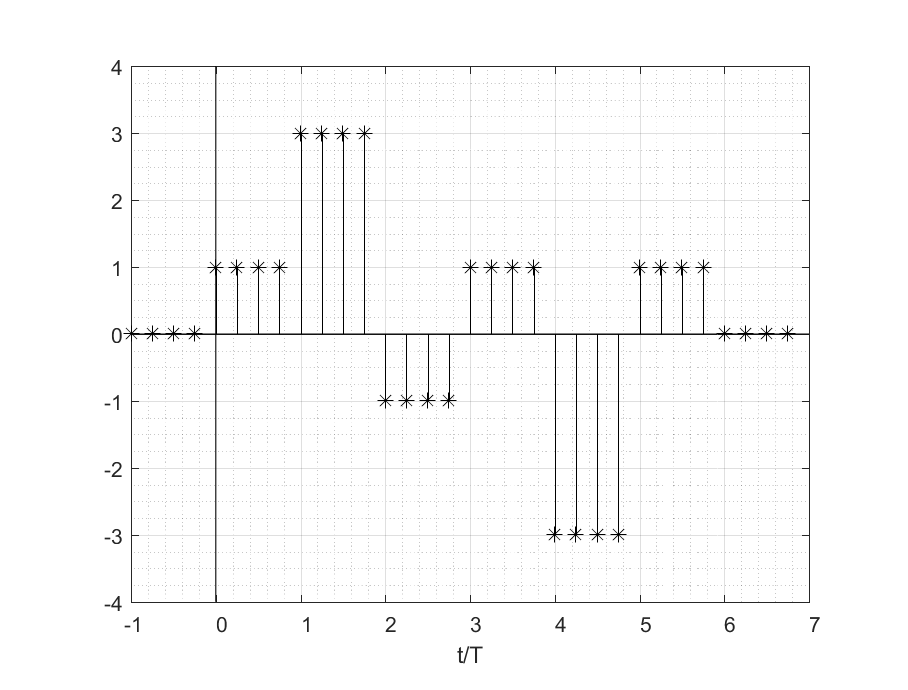
\includegraphics{pam001b}}
\caption{Firkantformet puls}
\end{subfigure}
\begin{subfigure}[b]{0.48\textwidth}
\centering\scalebox{0.53}{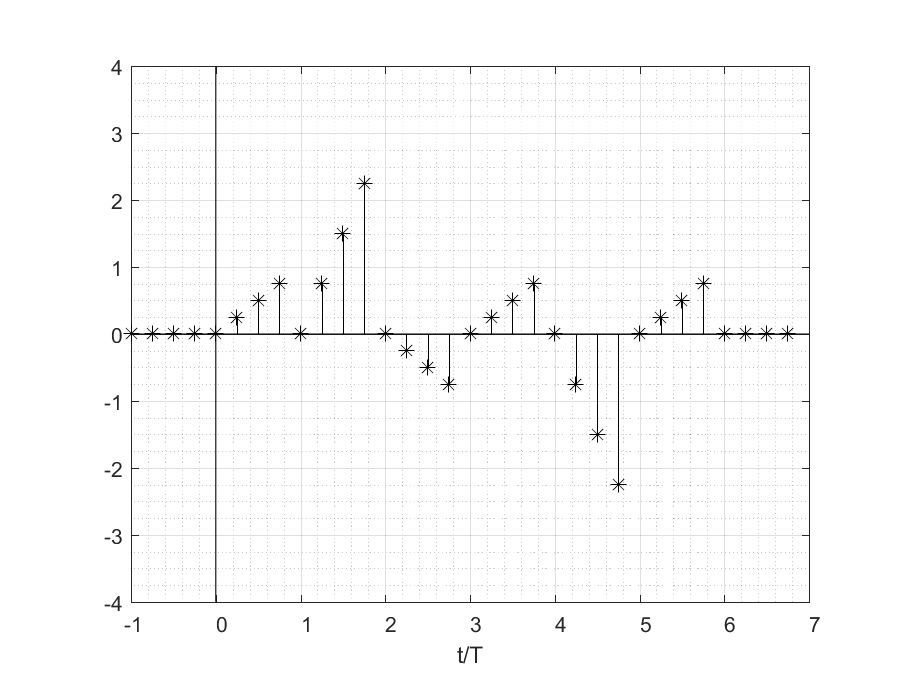
\includegraphics{pam001d}}
\caption{Savtakformet puls}
\end{subfigure}
\caption{\label{fig:pam001bd}Tidsdiskrete PAM-signaler.}
\end{figure}

%\noindent{}PAM-signaler kan også genereres med andet end firkantformede pulser. Figur~\ref{fig:pam001cd} illustrerer hhv. et kontinuert PAM-signal og det tilhørende tidsdiskrete for samme informationssekvens, $a_k$, som ovenfor, men nu med en ''savtakket'' pulsform.
%\begin{figure}[htbp]
%\centering
%\begin{subfigure}{.48\textwidth}
%\scalebox{0.5}{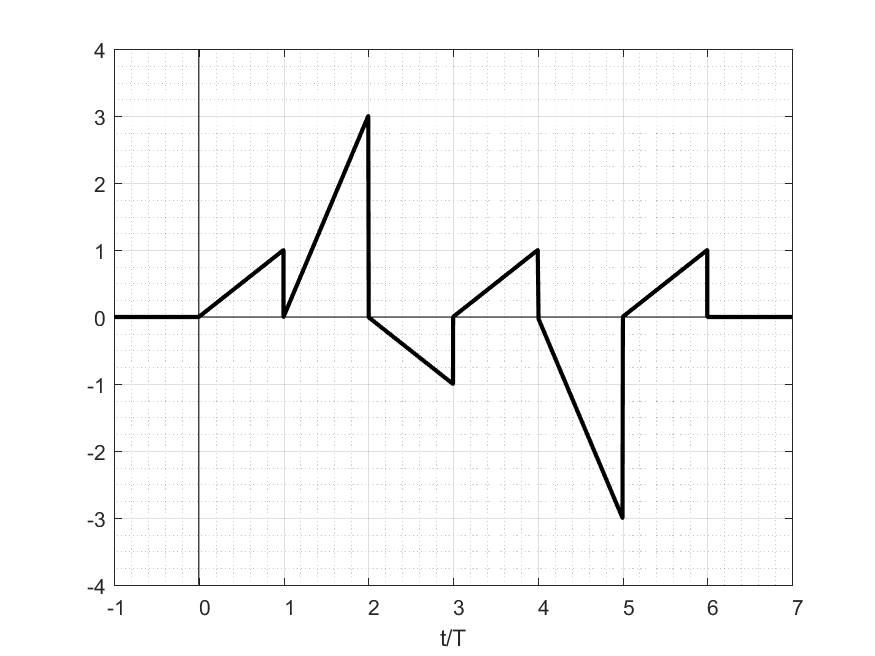
\includegraphics{pam001c}}
%\subcaption{Kontinuert PAM-signal}
%\end{subfigure}\hfill
%\begin{subfigure}{.48\textwidth}
%\scalebox{0.5}{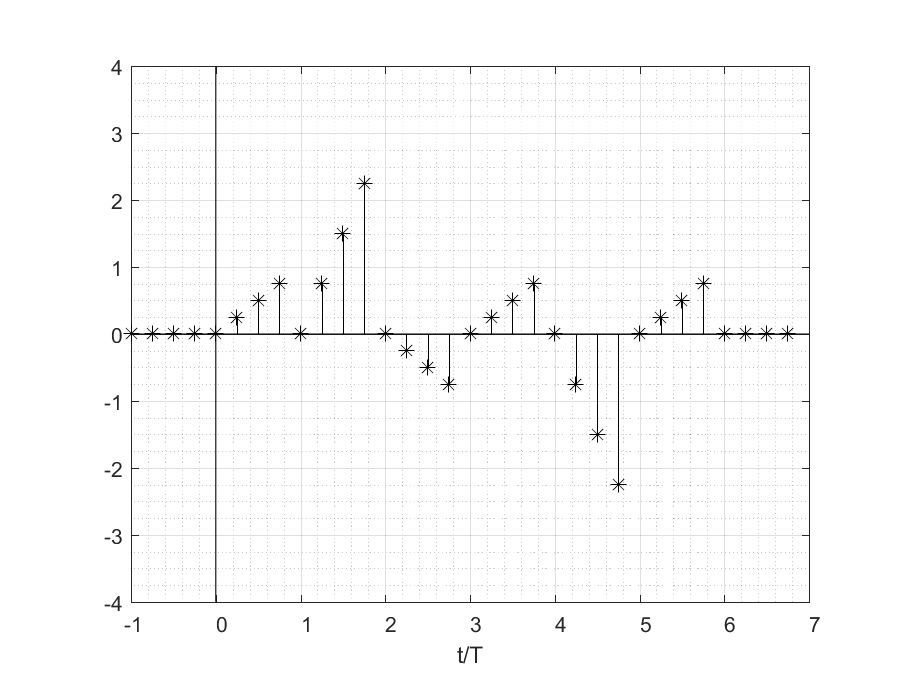
\includegraphics{pam001d}}
%\subcaption{Tidsdiskret PAM-signal}
%\end{subfigure}
%\caption{\label{fig:pam001cd}PAM-signaler med savtak-formet puls.}
%\end{figure}

\noindent{}I praksis vil samplingsintervallet, $T_s$, være valgt så $T_s = T/m \Leftrightarrow{} T = m \cdot T_s$ ($m \in \mathbb{N}$) for en passende værdi af $m$. Herved kan ligning~(\ref{eq:pamdiskret2}) omskrives
\begin{align}
v(n \cdot T_{s}) &= \sum_{k=0}^{\infty} a_{k} \cdot g(n \cdot T_{s}-k \cdot m \cdot T_s) \\
 &= \sum_{k=0}^{\infty} a_{k} \cdot g((n - k \cdot m) \cdot T_{s}) 
\end{align}

\noindent{}Indføres notationen $v_n$ som en kortere måde at skrive $v(n \cdot T_s)$ på (og tilsvarende mht. pulsen, dvs. $g_{n-k\cdot{}m} = g((n - k \cdot m) \cdot T_{s})$) fås:
\begin{equation}
v_n = \sum_{k=0}^{\infty} a_{k} \cdot g_{n - k \cdot m}
\label{eq:pamdiskret}
\end{equation}

\noindent{}Hvis man herefter opskriver leddene i summen i formel~(\ref{eq:pamdiskret}) ud fås
\begin{equation}
v_{n} = a_{0}\cdot{}g_{n} + a_{1}\cdot{}g_{n-m} + a_{2}\cdot{}g_{n-2m} + \ldots{} 
\label{eq:v_n}
\end{equation}

\section{Foldningsfunktionen}
Matematisk defineres {\em foldningen} af to tidsdiskrete sekvenser som vist i ligning~(\ref{eq:mathconv}) (hvoraf den ene sekvens blot er $g_k$-sekvensen som ovenfor)
\begin{equation}
y_n = \sum_{l=0}^{\infty} b_{l} \cdot g_{n-l}
\label{eq:mathconv}
\end{equation}

\noindent{}Det ses, at ligningerne~(\ref{eq:pamdiskret}) og~(\ref{eq:mathconv}) har næsten samme form, og da MATLAB har en indbygget funktion, kaldet \texttt{conv()}, der implementerer\footnote{I MATLAB vil der naturligvis være tale om, at både $b$- og $g$-sekvenserne har en endelig længde, men det er faktisk ikke nødvendigt i formel~(\ref{eq:mathconv}).}  ligning~(\ref{eq:mathconv}), er det nærliggende at forsøge at omskrive ligning~(\ref{eq:pamdiskret}), så den har samme form som ligning~(\ref{eq:mathconv}), så et PAM-signal i MATLAB kan genereres via MATLAB's \texttt{conv()}-funktion.

Hvis man tilføjer nogle led med værdien 0 til ligning~(\ref{eq:v_n}) fås
\begin{multline}
v_{n} = a_{0}\cdot{}g_{n} + 0\cdot{}g_{n-1} + 0\cdot{}g_{n-2} + \ldots + 0\cdot{}g_{n-(m-1)} +  \\
a_{1}\cdot{}g_{n-m} + 0\cdot{}g_{n-m-1} + 0\cdot{}g_{n-m-2} + \ldots + 0\cdot{}g_{n-(2m-1)} +  \\
a_{2}\cdot{}g_{n-2m} + 0\cdot{}g_{n-2m-1} + 0\cdot{}g_{n-2m-2} + \ldots + 0\cdot{}g_{n-(3m-1)} +  \\
a_{3}\cdot{}g_{n-3m} + 0\cdot{}g_{n-3m-1} + 0\cdot{}g_{n-3m-2} + \ldots + 0\cdot{}g_{n-(4m-1)} + \ldots{}
\label{eq:v_n2}
\end{multline}

\noindent{}Hvis man herefter \emph{definerer} en anden diskret sekvens, $b_l$ på følgende måde:
\begin{equation}
b_{l}=\left\lbrace
\begin{array}{ll}
a_{l/m} & \textrm{for }l=k\cdot{}m\textrm{ hvor }(k\in{}\mathbb{N}_{0}) \\
 & \\
0 & \textrm{ellers}\\
\end{array}
\right.
\label{eq:bseq}
\end{equation}
kan ligning~(\ref{eq:v_n2}) omskrives som
\begin{equation}
v_n=\sum_{l=0}^{\infty} b_l\cdot{}g_{n-l}
\label{eq:v_n3}
\end{equation}
som netop er identisk ved udtrykket for foldningen i ligning~(\ref{eq:mathconv}). Dvs. et PAM-signal kan dannes i MATLAB ved hjælp af en foldning, dvs. ved hjælp af MATLAB's \texttt{conv()}-funktion, når bare man har bestemt $b_l$ sekvensen på baggrund af $a_k$ sekvensen.

Ud fra ligning~(\ref{eq:bseq}) vil de første elementer i $b_l$ sekvensen være:
\begin{align*}
b_{0}&=a_{0},\\
b_{1}&=b_{2}=\ldots{}=b_{m-1}=0,\\
b_{m}&=a_{1},\\
b_{m+1}&=b_{m+2}=\ldots{}=b_{2m-1}=0,\\
b_{2m}&=a_{2}\\
&\vdots
\end{align*}
dvs. $b_l$-sekvensen dannes ved at der indsættes $m-1$ '0'-værdier efter hver $a_k$-værdi, dvs. som
\[
a_0,0,0,\ldots,0,a_1,0,0,\ldots,0,a_2,0,0,\ldots
\]

\noindent{}Dvs. det er muligt at generere et PAM-signal i MATLAB på flg. måde:
\begin{enumerate}
\item Lav en \emph{opsamplet} version, kaldet $au_l$ (som svarer til $b_l$-sekvensen ovenfor), af $a_k$-sekvensen ved at indsætte $m-1$ 0-værdier efter hver værdi fra $a_k$-sekvensen.
\item Udregn foldningen af $au_l$ og $g_l$ via MATLAB's \texttt{conv()}-funktion
\end{enumerate}

\noindent{}Dvs. flg. MATLAB kode kan benyttes til at generere et pulstog:
\begin{verbatim}
a = ...;  % Informationssekvens
m = ...;  % Antallet af samples pr. symbolperiode
g = ...;  % Udtryk for pulsformen
au = reshape([a; zeros(m-1,length(a))],1,[]);  % Upsamplet version af a-sekvens
v = conv(au,g);
\end{verbatim}

\noindent{}Efter denne MATLAB-kode vil rækkevektoren, \texttt{v}, indeholde den samplede udgave af PAM-signalet.

\end{document}
